\begin{frame}[fragile]{Visualização do {\it quicksort}}

    \begin{figure}
        \centering

        \begin{tikzpicture}
            \draw (0, 5) grid (9, 6);
            \draw[opacity=0] (0, 3) grid (9, 4);
            \draw[opacity=0] (0, 1) grid (9, 2);
            \draw[opacity=0] (0, -1) grid (9, 0);

            \draw[opacity=0] (0, -2) rectangle (1,-1);
            \draw[opacity=0,->] (3.5,4.5) node[anchor=north] { $p$ } -- (3.5,4.9);
            \draw[opacity=0,->] (3.5,-1.5) node[anchor=north] { $p$ } -- (3.5,-1.1);

            \node at (0.5, 5.5) { \textcolor{black}{$89$} };
            \node at (1.5, 5.5) { \textcolor{black}{$60$} };
            \node at (2.5, 5.5) { \textcolor{black}{$12$} };
            \node at (3.5, 5.5) { \textcolor{black}{$45$} };
            \node at (4.5, 5.5) { \textcolor{black}{$37$} };
            \node at (5.5, 5.5) { \textcolor{black}{$52$} };
            \node at (6.5, 5.5) { \textcolor{black}{$33$} };
            \node at (7.5, 5.5) { \textcolor{black}{$97$} };
            \node at (8.5, 5.5) { \textcolor{black}{$20$} };

        \end{tikzpicture}

    \end{figure}

\end{frame}

\begin{frame}[fragile]{Visualização do {\it quicksort}}

    \begin{figure}
        \centering

        \begin{tikzpicture}
            \draw (0, 5) grid (9, 6);
            \draw[opacity=0] (0, 3) grid (9, 4);
            \draw[opacity=0] (0, 1) grid (9, 2);
            \draw[opacity=0] (0, -1) grid (9, 0);

            \draw[opacity=0] (0, -2) rectangle (1,-1);
            \draw[opacity=1,->] (3.5,4.5) node[anchor=north] { $p$ } -- (3.5,4.9);
            \draw[opacity=0,->] (3.5,-1.5) node[anchor=north] { $p$ } -- (3.5,-1.1);

            \node at (0.5, 5.5) { \textcolor{black}{$89$} };
            \node at (1.5, 5.5) { \textcolor{black}{$60$} };
            \node at (2.5, 5.5) { \textcolor{black}{$12$} };
            \node at (3.5, 5.5) { \textcolor{black}{$45$} };
            \node at (4.5, 5.5) { \textcolor{black}{$37$} };
            \node at (5.5, 5.5) { \textcolor{black}{$52$} };
            \node at (6.5, 5.5) { \textcolor{black}{$33$} };
            \node at (7.5, 5.5) { \textcolor{black}{$97$} };
            \node at (8.5, 5.5) { \textcolor{black}{$20$} };

        \end{tikzpicture}

    \end{figure}

\end{frame}

\begin{frame}[fragile]{Visualização do {\it quicksort}}

    \begin{figure}
        \centering

        \begin{tikzpicture}
            \draw (0, 5) grid (9, 6);
            \draw[opacity=1] (0, 3) grid (9, 4);
            \draw[opacity=0] (0, 1) grid (9, 2);
            \draw[opacity=0] (0, -1) grid (9, 0);

            \draw[opacity=0] (0, -2) rectangle (1,-1);
            \draw[opacity=1,->] (3.5,4.5) node[anchor=north] { $p$ } -- (3.5,4.9);
            \draw[opacity=0,->] (3.5,-1.5) node[anchor=north] { $p$ } -- (3.5,-1.1);

            \node at (0.5, 5.5) { \textcolor{black}{$89$} };
            \node at (1.5, 5.5) { \textcolor{black}{$60$} };
            \node at (2.5, 5.5) { \textcolor{black}{$12$} };
            \node at (3.5, 5.5) { \textcolor{black}{$45$} };
            \node at (4.5, 5.5) { \textcolor{black}{$37$} };
            \node at (5.5, 5.5) { \textcolor{black}{$52$} };
            \node at (6.5, 5.5) { \textcolor{black}{$33$} };
            \node at (7.5, 5.5) { \textcolor{black}{$97$} };
            \node at (8.5, 5.5) { \textcolor{black}{$20$} };

            \node at (0.5, 3.5) { \textcolor{black}{$20$} };
            \node at (1.5, 3.5) { \textcolor{black}{$12$} };
            \node at (2.5, 3.5) { \textcolor{black}{$37$} };
            \node at (3.5, 3.5) { \textcolor{black}{$33$} };
            \node at (4.5, 3.5) { \textcolor{blue}{$\mathbf{45}$} };
            \node at (5.5, 3.5) { \textcolor{black}{$52$} };
            \node at (6.5, 3.5) { \textcolor{black}{$89$} };
            \node at (7.5, 3.5) { \textcolor{black}{$97$} };
            \node at (8.5, 3.5) { \textcolor{black}{$60$} };

        \end{tikzpicture}

    \end{figure}

\end{frame}

\begin{frame}[fragile]{Visualização do {\it quicksort}}

    \begin{figure}
        \centering

        \begin{tikzpicture}
            \draw (0, 5) grid (9, 6);
            \draw[opacity=1] (0, 3) grid (9, 4);
            \draw[opacity=0] (0, 1) grid (9, 2);
            \draw[opacity=0] (0, -1) grid (9, 0);

            \draw[opacity=0] (0, -2) rectangle (1,-1);
            \draw[opacity=1,->] (0.5,2.5) node[anchor=north] { $p$ } -- (0.5,2.9);
            \draw[opacity=1,->] (6.5,2.5) node[anchor=north] { $p$ } -- (6.5,2.9);

            \node at (0.5, 5.5) { \textcolor{black}{$89$} };
            \node at (1.5, 5.5) { \textcolor{black}{$60$} };
            \node at (2.5, 5.5) { \textcolor{black}{$12$} };
            \node at (3.5, 5.5) { \textcolor{black}{$45$} };
            \node at (4.5, 5.5) { \textcolor{black}{$37$} };
            \node at (5.5, 5.5) { \textcolor{black}{$52$} };
            \node at (6.5, 5.5) { \textcolor{black}{$33$} };
            \node at (7.5, 5.5) { \textcolor{black}{$97$} };
            \node at (8.5, 5.5) { \textcolor{black}{$20$} };

            \node at (0.5, 3.5) { \textcolor{black}{$20$} };
            \node at (1.5, 3.5) { \textcolor{black}{$12$} };
            \node at (2.5, 3.5) { \textcolor{black}{$37$} };
            \node at (3.5, 3.5) { \textcolor{black}{$33$} };
            \node at (4.5, 3.5) { \textcolor{blue}{$45$} };
            \node at (5.5, 3.5) { \textcolor{black}{$52$} };
            \node at (6.5, 3.5) { \textcolor{black}{$89$} };
            \node at (7.5, 3.5) { \textcolor{black}{$97$} };
            \node at (8.5, 3.5) { \textcolor{black}{$60$} };

        \end{tikzpicture}

    \end{figure}

\end{frame}

\begin{frame}[fragile]{Visualização do {\it quicksort}}

    \begin{figure}
        \centering

        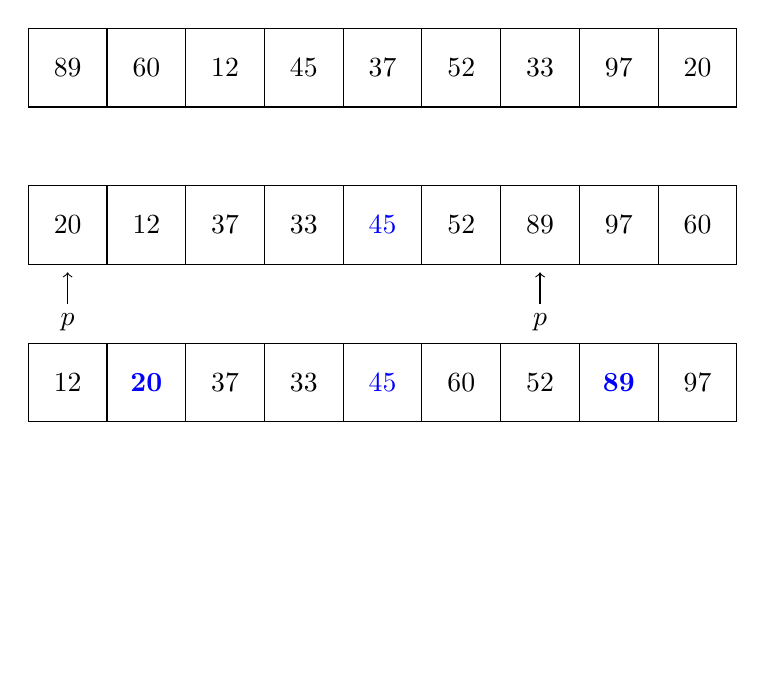
\begin{tikzpicture}
            \draw (0, 5) grid (9, 6);
            \draw[opacity=1] (0, 3) grid (9, 4);
            \draw[opacity=1] (0, 1) grid (9, 2);
            \draw[opacity=0] (0, -1) grid (9, 0);

            \draw[opacity=0] (0, -2) rectangle (1,-1);
            \draw[opacity=1,->] (0.5,2.5) node[anchor=north] { $p$ } -- (0.5,2.9);
            \draw[opacity=1,->] (6.5,2.5) node[anchor=north] { $p$ } -- (6.5,2.9);

            \node at (0.5, 5.5) { \textcolor{black}{$89$} };
            \node at (1.5, 5.5) { \textcolor{black}{$60$} };
            \node at (2.5, 5.5) { \textcolor{black}{$12$} };
            \node at (3.5, 5.5) { \textcolor{black}{$45$} };
            \node at (4.5, 5.5) { \textcolor{black}{$37$} };
            \node at (5.5, 5.5) { \textcolor{black}{$52$} };
            \node at (6.5, 5.5) { \textcolor{black}{$33$} };
            \node at (7.5, 5.5) { \textcolor{black}{$97$} };
            \node at (8.5, 5.5) { \textcolor{black}{$20$} };

            \node at (0.5, 3.5) { \textcolor{black}{$20$} };
            \node at (1.5, 3.5) { \textcolor{black}{$12$} };
            \node at (2.5, 3.5) { \textcolor{black}{$37$} };
            \node at (3.5, 3.5) { \textcolor{black}{$33$} };
            \node at (4.5, 3.5) { \textcolor{blue}{$45$} };
            \node at (5.5, 3.5) { \textcolor{black}{$52$} };
            \node at (6.5, 3.5) { \textcolor{black}{$89$} };
            \node at (7.5, 3.5) { \textcolor{black}{$97$} };
            \node at (8.5, 3.5) { \textcolor{black}{$60$} };

            \node at (0.5, 1.5) { \textcolor{black}{$12$} };
            \node at (1.5, 1.5) { \textcolor{blue}{$\mathbf{20}$} };
            \node at (2.5, 1.5) { \textcolor{black}{$37$} };
            \node at (3.5, 1.5) { \textcolor{black}{$33$} };
            \node at (4.5, 1.5) { \textcolor{blue}{$45$} };
            \node at (5.5, 1.5) { \textcolor{black}{$60$} };
            \node at (6.5, 1.5) { \textcolor{black}{$52$} };
            \node at (7.5, 1.5) { \textcolor{blue}{$\mathbf{89}$} };
            \node at (8.5, 1.5) { \textcolor{black}{$97$} };

        \end{tikzpicture}

    \end{figure}

\end{frame}

\begin{frame}[fragile]{Visualização do {\it quicksort}}

    \begin{figure}
        \centering

        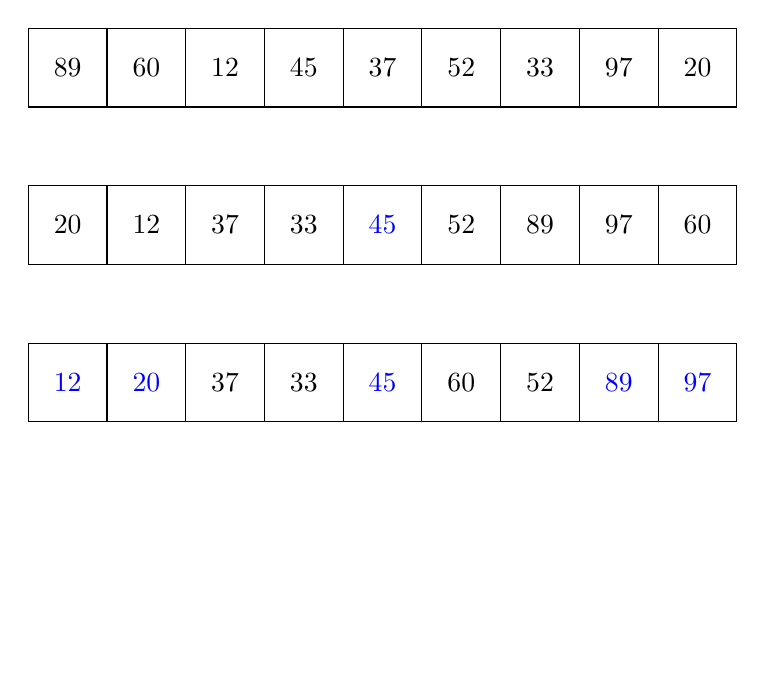
\begin{tikzpicture}
            \draw (0, 5) grid (9, 6);
            \draw[opacity=1] (0, 3) grid (9, 4);
            \draw[opacity=1] (0, 1) grid (9, 2);
            \draw[opacity=0] (0, -1) grid (9, 0);

            \draw[opacity=0] (0, -2) rectangle (1,-1);
            \draw[opacity=0,->] (0.5,2.5) node[anchor=north] { $p$ } -- (0.5,2.9);
            \draw[opacity=0,->] (6.5,2.5) node[anchor=north] { $p$ } -- (6.5,2.9);

            \node at (0.5, 5.5) { \textcolor{black}{$89$} };
            \node at (1.5, 5.5) { \textcolor{black}{$60$} };
            \node at (2.5, 5.5) { \textcolor{black}{$12$} };
            \node at (3.5, 5.5) { \textcolor{black}{$45$} };
            \node at (4.5, 5.5) { \textcolor{black}{$37$} };
            \node at (5.5, 5.5) { \textcolor{black}{$52$} };
            \node at (6.5, 5.5) { \textcolor{black}{$33$} };
            \node at (7.5, 5.5) { \textcolor{black}{$97$} };
            \node at (8.5, 5.5) { \textcolor{black}{$20$} };

            \node at (0.5, 3.5) { \textcolor{black}{$20$} };
            \node at (1.5, 3.5) { \textcolor{black}{$12$} };
            \node at (2.5, 3.5) { \textcolor{black}{$37$} };
            \node at (3.5, 3.5) { \textcolor{black}{$33$} };
            \node at (4.5, 3.5) { \textcolor{blue}{$45$} };
            \node at (5.5, 3.5) { \textcolor{black}{$52$} };
            \node at (6.5, 3.5) { \textcolor{black}{$89$} };
            \node at (7.5, 3.5) { \textcolor{black}{$97$} };
            \node at (8.5, 3.5) { \textcolor{black}{$60$} };

            \node at (0.5, 1.5) { \textcolor{blue}{$12$} };
            \node at (1.5, 1.5) { \textcolor{blue}{$20$} };
            \node at (2.5, 1.5) { \textcolor{black}{$37$} };
            \node at (3.5, 1.5) { \textcolor{black}{$33$} };
            \node at (4.5, 1.5) { \textcolor{blue}{$45$} };
            \node at (5.5, 1.5) { \textcolor{black}{$60$} };
            \node at (6.5, 1.5) { \textcolor{black}{$52$} };
            \node at (7.5, 1.5) { \textcolor{blue}{$89$} };
            \node at (8.5, 1.5) { \textcolor{blue}{$97$} };

        \end{tikzpicture}

    \end{figure}

\end{frame}

\begin{frame}[fragile]{Visualização do {\it quicksort}}

    \begin{figure}
        \centering

        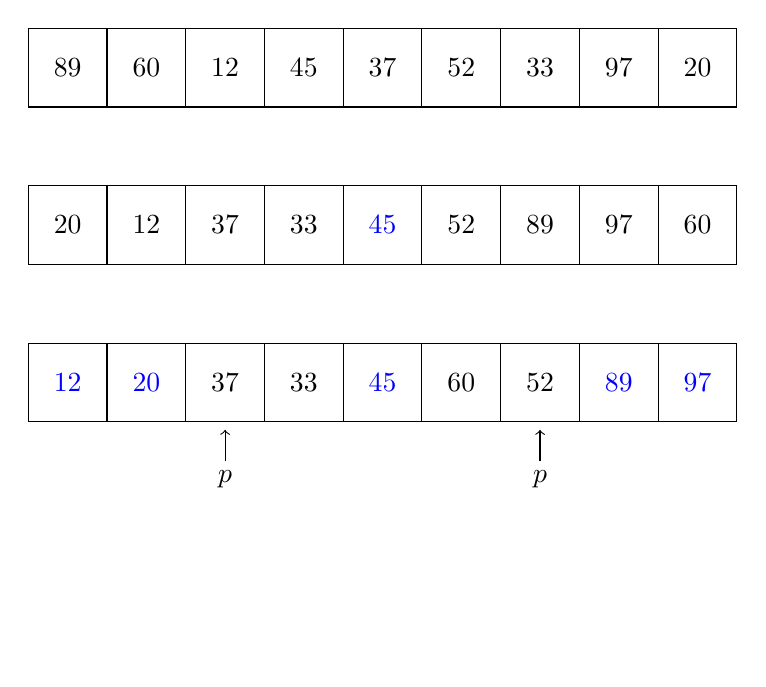
\begin{tikzpicture}
            \draw (0, 5) grid (9, 6);
            \draw[opacity=1] (0, 3) grid (9, 4);
            \draw[opacity=1] (0, 1) grid (9, 2);
            \draw[opacity=0] (0, -1) grid (9, 0);

            \draw[opacity=0] (0, -2) rectangle (1,-1);
            \draw[opacity=1,->] (2.5,0.5) node[anchor=north] { $p$ } -- (2.5,0.9);
            \draw[opacity=1,->] (6.5,0.5) node[anchor=north] { $p$ } -- (6.5,0.9);

            \node at (0.5, 5.5) { \textcolor{black}{$89$} };
            \node at (1.5, 5.5) { \textcolor{black}{$60$} };
            \node at (2.5, 5.5) { \textcolor{black}{$12$} };
            \node at (3.5, 5.5) { \textcolor{black}{$45$} };
            \node at (4.5, 5.5) { \textcolor{black}{$37$} };
            \node at (5.5, 5.5) { \textcolor{black}{$52$} };
            \node at (6.5, 5.5) { \textcolor{black}{$33$} };
            \node at (7.5, 5.5) { \textcolor{black}{$97$} };
            \node at (8.5, 5.5) { \textcolor{black}{$20$} };

            \node at (0.5, 3.5) { \textcolor{black}{$20$} };
            \node at (1.5, 3.5) { \textcolor{black}{$12$} };
            \node at (2.5, 3.5) { \textcolor{black}{$37$} };
            \node at (3.5, 3.5) { \textcolor{black}{$33$} };
            \node at (4.5, 3.5) { \textcolor{blue}{$45$} };
            \node at (5.5, 3.5) { \textcolor{black}{$52$} };
            \node at (6.5, 3.5) { \textcolor{black}{$89$} };
            \node at (7.5, 3.5) { \textcolor{black}{$97$} };
            \node at (8.5, 3.5) { \textcolor{black}{$60$} };

            \node at (0.5, 1.5) { \textcolor{blue}{$12$} };
            \node at (1.5, 1.5) { \textcolor{blue}{$20$} };
            \node at (2.5, 1.5) { \textcolor{black}{$37$} };
            \node at (3.5, 1.5) { \textcolor{black}{$33$} };
            \node at (4.5, 1.5) { \textcolor{blue}{$45$} };
            \node at (5.5, 1.5) { \textcolor{black}{$60$} };
            \node at (6.5, 1.5) { \textcolor{black}{$52$} };
            \node at (7.5, 1.5) { \textcolor{blue}{$89$} };
            \node at (8.5, 1.5) { \textcolor{blue}{$97$} };

        \end{tikzpicture}

    \end{figure}

\end{frame}

\begin{frame}[fragile]{Visualização do {\it quicksort}}

    \begin{figure}
        \centering

        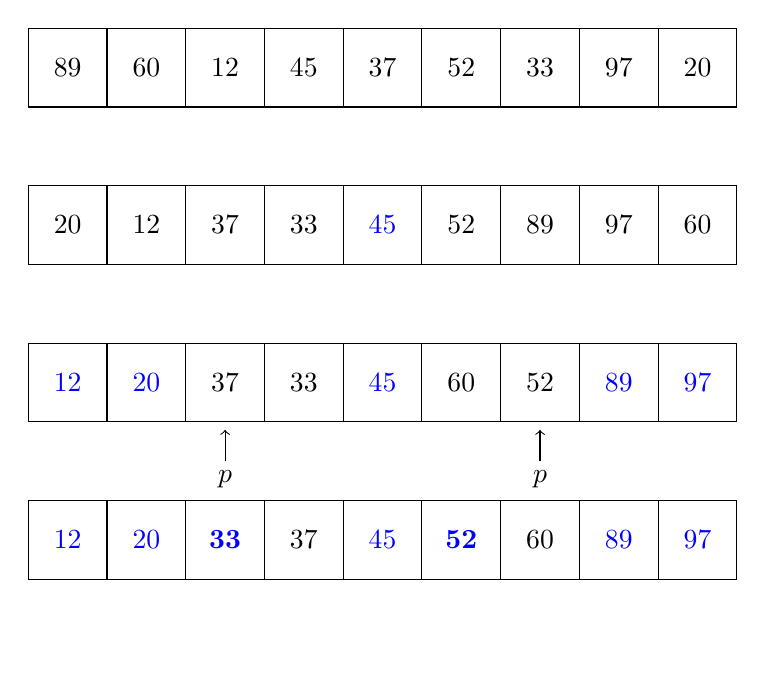
\begin{tikzpicture}
            \draw (0, 5) grid (9, 6);
            \draw[opacity=1] (0, 3) grid (9, 4);
            \draw[opacity=1] (0, 1) grid (9, 2);
            \draw[opacity=1] (0, -1) grid (9, 0);

            \draw[opacity=0] (0, -2) rectangle (1,-1);
            \draw[opacity=1,->] (2.5,0.5) node[anchor=north] { $p$ } -- (2.5,0.9);
            \draw[opacity=1,->] (6.5,0.5) node[anchor=north] { $p$ } -- (6.5,0.9);

            \node at (0.5, 5.5) { \textcolor{black}{$89$} };
            \node at (1.5, 5.5) { \textcolor{black}{$60$} };
            \node at (2.5, 5.5) { \textcolor{black}{$12$} };
            \node at (3.5, 5.5) { \textcolor{black}{$45$} };
            \node at (4.5, 5.5) { \textcolor{black}{$37$} };
            \node at (5.5, 5.5) { \textcolor{black}{$52$} };
            \node at (6.5, 5.5) { \textcolor{black}{$33$} };
            \node at (7.5, 5.5) { \textcolor{black}{$97$} };
            \node at (8.5, 5.5) { \textcolor{black}{$20$} };

            \node at (0.5, 3.5) { \textcolor{black}{$20$} };
            \node at (1.5, 3.5) { \textcolor{black}{$12$} };
            \node at (2.5, 3.5) { \textcolor{black}{$37$} };
            \node at (3.5, 3.5) { \textcolor{black}{$33$} };
            \node at (4.5, 3.5) { \textcolor{blue}{$45$} };
            \node at (5.5, 3.5) { \textcolor{black}{$52$} };
            \node at (6.5, 3.5) { \textcolor{black}{$89$} };
            \node at (7.5, 3.5) { \textcolor{black}{$97$} };
            \node at (8.5, 3.5) { \textcolor{black}{$60$} };

            \node at (0.5, 1.5) { \textcolor{blue}{$12$} };
            \node at (1.5, 1.5) { \textcolor{blue}{$20$} };
            \node at (2.5, 1.5) { \textcolor{black}{$37$} };
            \node at (3.5, 1.5) { \textcolor{black}{$33$} };
            \node at (4.5, 1.5) { \textcolor{blue}{$45$} };
            \node at (5.5, 1.5) { \textcolor{black}{$60$} };
            \node at (6.5, 1.5) { \textcolor{black}{$52$} };
            \node at (7.5, 1.5) { \textcolor{blue}{$89$} };
            \node at (8.5, 1.5) { \textcolor{blue}{$97$} };

            \node at (0.5, -0.5) { \textcolor{blue}{$12$} };
            \node at (1.5, -0.5) { \textcolor{blue}{$20$} };
            \node at (2.5, -0.5) { \textcolor{blue}{$\mathbf{33}$} };
            \node at (3.5, -0.5) { \textcolor{black}{$37$} };
            \node at (4.5, -0.5) { \textcolor{blue}{$45$} };
            \node at (5.5, -0.5) { \textcolor{blue}{$\mathbf{52}$} };
            \node at (6.5, -0.5) { \textcolor{black}{$60$} };
            \node at (7.5, -0.5) { \textcolor{blue}{$89$} };
            \node at (8.5, -0.5) { \textcolor{blue}{$97$} };

        \end{tikzpicture}

    \end{figure}

\end{frame}

\begin{frame}[fragile]{Visualização do {\it quicksort}}

    \begin{figure}
        \centering

        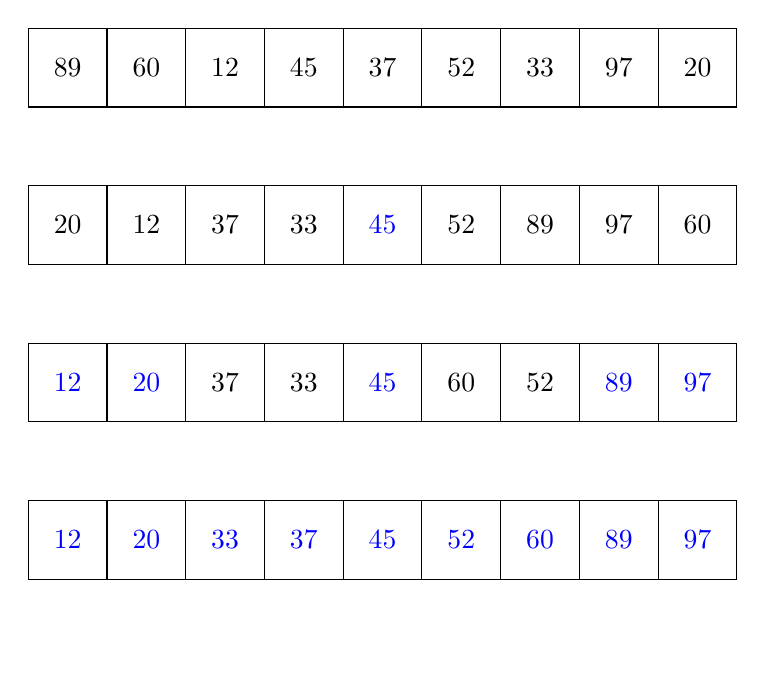
\begin{tikzpicture}
            \draw (0, 5) grid (9, 6);
            \draw[opacity=1] (0, 3) grid (9, 4);
            \draw[opacity=1] (0, 1) grid (9, 2);
            \draw[opacity=1] (0, -1) grid (9, 0);

            \draw[opacity=0] (0, -2) rectangle (1,-1);
            \draw[opacity=0,->] (2.5,0.5) node[anchor=north] { $p$ } -- (2.5,0.9);
            \draw[opacity=0,->] (6.5,0.5) node[anchor=north] { $p$ } -- (6.5,0.9);

            \node at (0.5, 5.5) { \textcolor{black}{$89$} };
            \node at (1.5, 5.5) { \textcolor{black}{$60$} };
            \node at (2.5, 5.5) { \textcolor{black}{$12$} };
            \node at (3.5, 5.5) { \textcolor{black}{$45$} };
            \node at (4.5, 5.5) { \textcolor{black}{$37$} };
            \node at (5.5, 5.5) { \textcolor{black}{$52$} };
            \node at (6.5, 5.5) { \textcolor{black}{$33$} };
            \node at (7.5, 5.5) { \textcolor{black}{$97$} };
            \node at (8.5, 5.5) { \textcolor{black}{$20$} };

            \node at (0.5, 3.5) { \textcolor{black}{$20$} };
            \node at (1.5, 3.5) { \textcolor{black}{$12$} };
            \node at (2.5, 3.5) { \textcolor{black}{$37$} };
            \node at (3.5, 3.5) { \textcolor{black}{$33$} };
            \node at (4.5, 3.5) { \textcolor{blue}{$45$} };
            \node at (5.5, 3.5) { \textcolor{black}{$52$} };
            \node at (6.5, 3.5) { \textcolor{black}{$89$} };
            \node at (7.5, 3.5) { \textcolor{black}{$97$} };
            \node at (8.5, 3.5) { \textcolor{black}{$60$} };

            \node at (0.5, 1.5) { \textcolor{blue}{$12$} };
            \node at (1.5, 1.5) { \textcolor{blue}{$20$} };
            \node at (2.5, 1.5) { \textcolor{black}{$37$} };
            \node at (3.5, 1.5) { \textcolor{black}{$33$} };
            \node at (4.5, 1.5) { \textcolor{blue}{$45$} };
            \node at (5.5, 1.5) { \textcolor{black}{$60$} };
            \node at (6.5, 1.5) { \textcolor{black}{$52$} };
            \node at (7.5, 1.5) { \textcolor{blue}{$89$} };
            \node at (8.5, 1.5) { \textcolor{blue}{$97$} };

            \node at (0.5, -0.5) { \textcolor{blue}{$12$} };
            \node at (1.5, -0.5) { \textcolor{blue}{$20$} };
            \node at (2.5, -0.5) { \textcolor{blue}{$33$} };
            \node at (3.5, -0.5) { \textcolor{blue}{$37$} };
            \node at (4.5, -0.5) { \textcolor{blue}{$45$} };
            \node at (5.5, -0.5) { \textcolor{blue}{$52$} };
            \node at (6.5, -0.5) { \textcolor{blue}{$60$} };
            \node at (7.5, -0.5) { \textcolor{blue}{$89$} };
            \node at (8.5, -0.5) { \textcolor{blue}{$97$} };

        \end{tikzpicture}

    \end{figure}

\end{frame}
